%%%%%%%%%%%%%%%%%%%%%%%%%%%%%%%%%%%%%%%%%%%%%%%%%%%%%%%%%%%%%%%%%%%%%%%%%%%%%%%%%%%%%%%%%%%%%%%%%%%
\documentclass[10pt, a4paper]{article}
%%%%%%%%%%%%%%%%%%%%%%%%%%%%%%%%%%%%%%%%%%%%%%%%%%%%%%%%%%%%%%%%%%%%%%%%%%%%%%%%%%%%%%%%%%%%%%%%%%%

%--------------------------------------------------------------------------------------------------
% Dimensions :
%--------------------------------------------------------------------------------------------------

\setlength{\textheight}{26cm}
\setlength{\textwidth}{16cm}

\setlength{\topmargin}{-25mm}
\setlength{\oddsidemargin}{0mm}
\setlength{\evensidemargin}{0mm}

% \setlength{\columnsep}{20mm}

\setlength{\fboxsep}{1mm}
\setlength{\unitlength}{1mm}

%--------------------------------------------------------------------------------------------------
% Packages :
%--------------------------------------------------------------------------------------------------

\usepackage{latexsym}
\usepackage{graphicx}
\usepackage{pifont}
\usepackage{color}
\usepackage{amsmath}
\usepackage{amssymb}
\usepackage{enumerate}

\usepackage[french]{babel}    % pour franciser le document

%\usepackage[latin1]{inputenc} % pour utiliser les caracteres accentues du claviers
\usepackage[utf8]{inputenc} 

\usepackage{accents}

\usepackage{cancel}
% Style des vecteurs : fleche ou gras ?

%\newcommand{\myvec}[1]{\boldsymbol{#1}}
\newcommand{\myvec}[1]{\vec{#1}}

\newcommand{\mytensor}[1]{\accentset{\Rightarrow}{#1}} % needs \usepackage{accents}

%---------------------------
% Operateurs differentiels :
%---------------------------

\newcommand{\divergence}{\mbox{\rm div}\,}

\newcommand{\gradient}{\myvec{\mbox{\rm gra}}\mbox{\rm d}}
% \newcommand{\gradient}{\mathbf{grad}\,}
% \newcommand{\ggradient}{\stackrel{\Rightarrow}{\mbox{gra}}\!\!\!\,\mbox{d}\,}
\newcommand{\ggradient}{\accentset{\Rightarrow}{\mbox{\rm gra}}\mbox{\rm d}\!}

%\renewcommand{\dot}[1]{\accentset{\hbox{\huge .}}{#1}}
\newcommand{\mydot}[1]{\accentset{\centerdot}{#1}}

\newcommand{\rot}{\vec{\mbox{\rm ro}}\mbox{\rm t}\,}
%\newcommand{\rot}{\mathbf{rot}\,}

% \newcommand{\vnabla}{\vec{\nabla}}
\newcommand{\vnabla}{\boldsymbol{\nabla}}

% Fonctions speciales:

\newcommand{\besselj}[1]{\mbox{J}_{#1}}
\newcommand{\besselk}[1]{\mbox{K}_{#1}}
\newcommand{\bessely}[1]{\mbox{Y}_{#1}}
\newcommand{\besseli}[1]{\mbox{I}_{#1}}

% Vecteurs, tenseurs et torseurs:

\newcommand{\ex}{\mathbf{e}_{x}}
\newcommand{\ey}{\mathbf{e}_{y}}
\newcommand{\ez}{\mathbf{e}_{z}}

\newcommand{\er}{\mathbf{e}_{r}}
\newcommand{\erho}{\mathbf{e}_{\rho}}
\newcommand{\ephi}{\mathbf{e}_{\varphi}}
\newcommand{\etheta}{\mathbf{e}_{\theta}}

%\newcommand{\tensor}[1]{\stackrel{\Rightarrow}{#1}}
\newcommand{\tensor}[1]{\mbox{\sl \textbf{#1}}}
\newcommand{\torseur}[4]{
   \!\!\!\! \left . \begin{array}{c} \\ \\ _#1 \end{array} \!\!\!
   \right \{ \!\!\!
   \begin{array}{#4} #2 \\ \\ #3 \end{array}}

% Integrales multiples:

\newcommand{\odblint}[1]{\int\!\!\!\!\!\int_{#1} \hskip -7mm \bigcirc \;}
\newcommand{\dblint}{\int\!\!\!\!\!\int}
\newcommand{\tplint}{\int\!\!\!\!\!\int\!\!\!\!\!\int}

% Fractions:

\renewcommand{\dfrac}[2]{\displaystyle \frac{#1}{#2}}

% Derivees ordinaires et partielles:

\newcommand{\dpdt}[1]{\dfrac{\partial #1}{\partial t}}
\newcommand{\dpdx}[1]{\dfrac{\partial #1}{\partial x}}
\newcommand{\dpdy}[1]{\dfrac{\partial #1}{\partial y}}
\newcommand{\dpdz}[1]{\dfrac{\partial #1}{\partial z}}

\newcommand{\ddpdt}[1]{\dfrac{\partial^2 #1}{\partial t^2}}
\newcommand{\ddpdx}[1]{\dfrac{\partial^2 #1}{\partial x^2}}
\newcommand{\ddpdy}[1]{\dfrac{\partial^2 #1}{\partial y^2}}
\newcommand{\ddpdz}[1]{\dfrac{\partial^2 #1}{\partial z^2}}

\newcommand{\dpdr}[1]{\dfrac{\partial #1}{\partial r}}
\newcommand{\dpdrho}[1]{\dfrac{\partial #1}{\partial \rho}}
\newcommand{\dpdphi}[1]{\dfrac{\partial #1}{\partial \varphi}}
\newcommand{\dpdtheta}[1]{\dfrac{\partial #1}{\partial \theta}}

\newcommand{\ddpdr}[1]{\dfrac{\partial^2 #1}{\partial r^2}}
\newcommand{\ddpdrho}[1]{\dfrac{\partial^2 #1}{\partial \rho^2}}
\newcommand{\ddpdphi}[1]{\dfrac{\partial^2 #1}{\partial \varphi^2}}
\newcommand{\ddpdtheta}[1]{\dfrac{\partial ^2#1}{\partial \theta^2}}

\newcommand{\ddt}[1]{\dfrac{d #1}{dt}}
\newcommand{\ddx}[1]{\dfrac{d #1}{dx}}
\newcommand{\ddy}[1]{\dfrac{d #1}{dy}}
\newcommand{\ddz}[1]{\dfrac{d #1}{dz}}
\newcommand{\ddr}[1]{\dfrac{d #1}{dr}}

\newcommand{\ddtref}[2]{\dfrac{d #1}{dt}_{\! | #2 }}
\newcommand{\dpdtref}[3]{\dfrac{\partial #1}{\partial #2}_{\! | #3 }}

% Misc:

\newcommand{\mycaption}[1]{\caption{\sl #1}}

\newcommand{\ligne}[1]{\hrule height #1\linethickness \hfill}

\newcommand{\thickline}[2]{\linethickness{#1} \line(1, 0){#2}}

\newcommand{\myline}{\noindent\underline{\hspace{\textwidth}}}
\newcommand{\mysection}[1]{\vskip 0.5cm \section{#1}\vskip -1.4cm 
   \myline \vskip 0.4cm \myline \bigskip}

\newcommand{\etal}{\textit{et al.}}

\newcommand{\varray}[1]{\renewcommand{\arraystretch}{#1}}

\newcommand{\puissance}[1]{^{\mbox{\footnotesize #1}}}
\newcommand{\indice}[1]{_{\mbox{\footnotesize #1}}}

%---------------------------------------------------------------------
% New environments:
%---------------------------------------------------------------------

\newcounter{MyEnumCounter}
\newcounter{MySaveCounter}
\newenvironment{MyEnum}{%
  \begin{list}{\arabic{MyEnumCounter}.}{\usecounter{MyEnumCounter}%
  \setcounter{MyEnumCounter}{\value{MySaveCounter}}}
  }{%
  \setcounter{MySaveCounter}{\value{MyEnumCounter}}\end{list}%
}
\newcommand{\MyEnumReset}{\setcounter{MySaveCounter}{0}}

\newenvironment{deuxcols}{\begin{tabular}{lr} \hspace*{-9.7mm}}{\end{tabular}}

\newenvironment{dem}{\noindent %
   \begin{tabular}{||l} \textsl{D\'emonstration :} \\ % 
   \begin{minipage}{15.5cm} \footnotesize} %
   {\end{minipage}\end{tabular}}

\newenvironment{abst}{\begin{quotation}\sl}{\end{quotation}}

\newenvironment{eqnbox}{\begin{equation}\begin{array}{|c|}  \hline \\ 
   \displaystyle}{\\ \\ \hline \end{array} \end{equation}}

\newcommand{\myprime}{\ \!'}

% JFM symbols:

\DeclareMathSymbol{\varGamma}{\mathord}{letters}{"00}
\DeclareMathSymbol{\varDelta}{\mathord}{letters}{"01}
\DeclareMathSymbol{\varTheta}{\mathord}{letters}{"02}
\DeclareMathSymbol{\varLambda}{\mathord}{letters}{"03}
\DeclareMathSymbol{\varXi}{\mathord}{letters}{"04}
\DeclareMathSymbol{\varPi}{\mathord}{letters}{"05}
\DeclareMathSymbol{\varSigma}{\mathord}{letters}{"06}
\DeclareMathSymbol{\varUpsilon}{\mathord}{letters}{"07}
\DeclareMathSymbol{\varPhi}{\mathord}{letters}{"08}
\DeclareMathSymbol{\varPsi}{\mathord}{letters}{"09}
\DeclareMathSymbol{\varOmega}{\mathord}{letters}{"0A}

% ---------------------------------------------------------------------
% MISC SYMBOLS :
% ---------------------------------------------------------------------

\font\SY=msam10 
\def\carreblanc{\hbox{\SY \char'3}}
\def\carrenoir{\hbox{\SY \char'4}}
\def\diamblanc{\hbox{\SY \char'6}}
\def\diamnoir{\hbox{\SY \char'7}}
\def\triblancright{\hbox{\SY \char'102}}
\def\triblancleft{\hbox{\SY \char'103}}
\def\triblancup{\hbox{\SY \char'115}}
\def\triblancdown{\hbox{\SY \char'117}}
\def\trinoirright{\hbox{\SY \char'111}}
\def\trinoirleft{\hbox{\SY \char'112}}
\def\trinoirup{\hbox{\SY \char'116}}
\def\trinoirdown{\hbox{\SY \char'110}}
\def\rondblanc{\hbox{\scriptsize $\bigcirc$}}
\def\rondnoir{\hbox{\LARGE $\bullet$}}

\font\BB=msbm10 scaled 1095
\def\setr{\hbox{\BB R}}
\def\setc{\hbox{\BB C}}
\def\setn{\hbox{\BB N}}
\def\setz{\hbox{\BB Z}}

% Pour enlever la numerotation des pages de la table des matieres:

%%%% debut macro, a placer dans preambule %%%%
\makeatletter
\def\addcontentsline@toc#1#2#3{%
   \addtocontents{#1}{\protect\thispagestyle{empty}}%
   \addtocontents{#1}{\protect\contentsline{#2}{#3}{\thepage}}}
\def\addcontentsline#1#2#3{%
  \expandafter\@ifundefined{addcontentsline@#1}%
  {\addtocontents{#1}{\protect\contentsline{#2}{#3}{\thepage}}}
  {\csname addcontentsline@#1\endcsname{#1}{#2}{#3}}}
\makeatother
%%%% fin macro %%%%

\newcommand{\titre}[1]{ %
  \medskip \noindent \underline{\makebox[\textwidth][l]{\textbf{#1}\textcolor{white}{pl}}}}% \\}

\newcommand{\sstitre}[1]{ %
  \bigskip \centerline{\textbf{#1}} \smallskip}

\def\draft{\overfullrule 5pt} % The \draft command marks the overful boxes

\def\indentlist{\list%
        {}{\labelwidth 0pt \leftmargin 3\labelsep}}
\let\endindentlist\endlist \relax

\def\datelist{\list%
        {}{\settowidth\labelwidth{[2001/02 :]}
        \leftmargin\labelwidth
        \advance\leftmargin\labelsep}
}
\let\enddatelist\endlist \relax

\def\longuelist{\list%
        {}{\settowidth\labelwidth{[Etablissement :]}
        \leftmargin\labelwidth
        \advance\leftmargin\labelsep}
}
\let\endlonguelist\endlist \relax

\def\shortlist{\list%
        {}{\settowidth\labelwidth{$\bullet$}
        \leftmargin\labelwidth
        \advance\leftmargin\labelsep}
}
\let\endshortlist\endlist \relax



%--------------------------------------------------------------------------------------------------
% Divers :
%--------------------------------------------------------------------------------------------------

\definecolor{rougefonce}{rgb}{0.7, 0.2, 0.2}

\renewcommand{\thickline}[2]{\linethickness{#1} \line(1, 0){#2}}
\renewcommand{\mycaption}[1]{\caption{\sl #1}}
\renewcommand{\myvec}[1]{\vec{#1}}

\newcommand{\footnoteremember}[2]{
\footnote{#2}
\newcounter{#1}
\setcounter{#1}{\value{footnote}}% \!\!\!
}
\newcommand{\footnoterecall}[1]{
\footnotemark[\value{#1}]
}

% \pagestyle{empty}

\graphicspath{{../FIGURES/}{Figures/}} % chemin d'acces au repertoire des figures (par ex.)

%%%%%%%%%%%%%%%%%%%%%%%%%%%%%%%%%%%%%%%%%%%%%%%%%%%%%%%%%%%%%%%%%%%%%%%%%%%%%%%%%%%%%%%%%%%%%%%%%%%
\begin{document}
%%%%%%%%%%%%%%%%%%%%%%%%%%%%%%%%%%%%%%%%%%%%%%%%%%%%%%%%%%%%%%%%%%%%%%%%%%%%%%%%%%%%%%%%%%%%%%%%%%%

\begin{center}

  \textsc{Université Toulouse 3 -- Paul Sabatier \hfill Année universitaire 2017-2018}
  
  \textsc{Mécanique des fluides \hfill L3 Mécanique}
  
  \vspace{0mm}
  
  \begin{center}
    \thickline{0.4mm}{160}
    \\ \vspace{3mm}
  \textbf{\large Exercice complémentaire 10 : 
  \\
  Réflexion/transmission d'une onde acoustique;  \\
  Application au fonctionnement de l'oreille moyenne}
    \\ %\vspace{1mm}
    \thickline{0.4mm}{160}
  \end{center}

  %\vspace{5mm}
  
\end{center}

\section{Description d'une onde acoustique monodimensionnelle}

On se place tout d'abord dans un milieu homogène, de propriétés thermodynamiques moyennes 
$\rho_0,p_0,T_0$ (on néglige la gravité).
On étudie la propagation d'ondes acoustiques monodimensionnelles, décrites par leur fluctuation de pression $p'(x,t)$ et fluctuation de vitesse $\vec{u}' =  u'(x,t) \vec{e}_x$.
 
\begin{enumerate}
\item Rappelez les hypothèses de l'acoustique linéaire. Montrez que sous ces hypothèses, l'évolution de la pression est gouvernée par l'équation de Helmholtz :

$$
\frac{\partial^2 p'}{\partial t^2} = c_0^2 \nabla^2 p'
$$

Définir $c_0$ dans le cas général, puis dans le cas d'un gaz parfait.

\item On considère une solution d'onde plane progressive monochromatique se déplaçant dans la direction $+\vec{e}_x$, sous la  forme suivante :
$$
p'(x,t) = Re (A e^{i (k x - \omega t)})
$$
Représentez la forme d'une telle onde à différents instants. 

A quoi correspondent les quantités $A$, $k$ et $\omega$ ? Quelle relation relie ces deux dernières quantités ?

\item A partir des équations du mouvement, donnez la loi de vitesse $u'(x,t)$ correspondant à une telle onde.

\item Définir l'énergie acoustique volumique $e_{ac}$ et le vecteur intensité acoustique $\vec{I}$. 

\item Montrez que dans le cas considéré ici, la valeur moyenne de ces quantités (au sens de la moyenne temporelle sur une période d'oscillation) sont données respectivement par :
 
$$
\overline{e_{ac}} = \frac{A^2}{2 \rho_0 c_0 ^2} ; \qquad \overline{I_x} = c_0  \overline{e_{ac}} 
$$

\item Comment faut-il modifier les relations données aux questions 2, 3 et 5 pour décrire une onde plane progressive monochromatique d'amplitude $B$ se déplaçant dans la direction $-\vec{e}_x$? 


\item {\em Question supplémentaire*}.
On reprend l'étude dans le cas d'un {\em solide élastique} de propriétés mécaniques $E$ (module d'Young), $\nu$ (coefficient de Poisson), $\rho_0$ (masse volumique).

Montrez qu'un milieu infini permet la propagation d'{\em ondes de compression} (qui généralisent les ondes acoustiques) avec une vitesse donnée par 
$$
c_l^2 = \frac{E(1-\nu)}{\rho (1+\nu)(1- 2 \nu)}.
$$


\section{Réflexion/transmission d'une onde acoustique}



On étudie la propagation d'ondes acoustiques dans un milieu composé de deux demi-espaces occupés par des fluides\footnote{Le cas ou l'un des milieux (ou les 2) est un solide élastique se traite de la même façon en remplaçant $c$ par $c_l$} de propriétés moyennes différentes, c'est-à-dire :
$$
(x<0 ) : \quad \rho_0 = \rho_1 ; c_0 = c_1 ; \quad \qquad (x>0 ) : \quad  \rho_0 = \rho_2 ; c_0 = c_2
$$
%On considère des ondes monodimensionelles de la forme : 
%$p' = p'(x,t)$ et $\vec{u'} = u'(x,t) \vec{e}_x$.

Dans les applications numériques, on considèrera que le milieu $1$ est de l'air ($\rho_1 = 1.225 kg/m^3 ; c_1 = 340 m/s$) et que le milieu $2$ est de l'eau 
($\rho_2 = 1000 kg/m^3 ; c_2 = 1500 m/s$).


 \item 
On suppose que le champ de pression est donné par une loi de la forme suivante (ou il est sous-entendu qu'il convient de ne retenir que la partie réelle des quantités complexes) :
\begin{equation}
p'(x,t) = \left\{ \begin{array}{ll} 
A e^{i (k_1 x - \omega t)} + B e^{i (-k_1 x - \omega t)} & \quad ( \mbox{ pour }  x<0) \\
C e^{i (k_2 x - \omega t)} & \quad ( \mbox{ pour }  x>0) 
\end{array}
\right.
\label{eq:ABC}
\end{equation}

Comment peut-on qualifier les 3 ondes d'amplitudes $A$, $B$, $C$ apparaissant dans cette expression ? Quelle est l'interprétation physique de cette situation ?

\item Quel est l'expression des paramètres $k_1$ et $k_2$ en fonction de la fréquence $\omega$ et des propriétés des milieux correspondant ?

Application numérique : donnez la valeur de $k_1$ et $k_2$ ainsi que les longueurs d'ondes associées $\lambda_1$, $\lambda_2$ pour une fréquence $\omega = 2 \pi f $ avec $f = 440 Hz$ (fréquence de la note de référence $la_4$ pour les instruments de musique) pour une transmission entre l'air et l'eau. 

\item
A partir des équations du mouvement, donnez l'expression du champ de vitesse $u'(x,t)$ (respectivement pour $x<0$ et pour $x>0$) .

\item 
Justifiez que la pression $p'$ et la vitesse $u'$ sont continues à l'interface entre les deux milieux 
(en $x=0$). En déduire un système de 2 équations pour les 2 inconnues $B$ et $C$ ($A$ étant supposé connu).

\item 
En déduire la valeur des coefficients de réflexion et de de transmission en amplitude-pression :
\begin{eqnarray}
r = \frac{B}{A} &=& \frac{\rho_2 c_2 - \rho_1 c_1}{\rho_1 c_1 + \rho_2 c_2},\\
t = \frac{C}{A} &=& \frac{2 \rho_2 c_2}{\rho_1 c_1 + \rho_2 c_2},
\label{eq:rt}
\end{eqnarray}


\item Montrez que les coefficients de réflexion et de transmission en énergie ont les expressions suivantes :
\begin{eqnarray}
R = r^2 &=& \left(\frac{\rho_1 c_1 - \rho_2 c_2}{\rho_1 c_1 + \rho_2 c_2}\right)^2,\\
T = \left( \frac{\rho_1 c_1}{\rho_2 c_2} \right) t^2 &=& \frac{4 \rho_1 c_1\rho_2 c_2}{(\rho_1 c_1 + \rho_2 c_2)^2}.
\label{eq:RT}
\end{eqnarray}
Vérifiez que $T+R = 1$. Quelle est l'interprétation physique de ce résultat ?

\item Application numérique : donnez les valeurs de $t,r,T,R$ pour la transmission entre l'air et l'eau.
Exprimez $T$ en décibels.

\item {\em Question supplémentaire*}.
On considère maintenant, non plus un milieu infini des deux côtés de la discontinuité, mais un conduit cylindrique d'axe $\vec{e}_x$, dont la section varie brutalement entre une valeur $S_1$ (pour $x<0$) et une valeur $S_2$ (pour $x>0$). On suppose que le champ de pression reste donné par la description (\ref{eq:ABC}).

On note $q'(x,t)  = u' S$ le débit de volume à travers la section du tube.

\begin{enumerate}

\item A partir des expressions de la question 10, donnez  l'expression de $q'(x,t)$, respectivement  pour $x<0$ et $x>0$.

\item
Montrez qu'a partir de la continuité de la pression et du débit en $x=0$ on obtient des formules qui généralisent les équations (2,3,4,5) %(\ref{eq:rt} et \ref{eq:RT}) 
en remplaçant $\rho_1 c_1$ par $Z_1 = \rho_1 c_1/S_1$ et  $\rho_2 c_2$ par $Z_2 = \rho_2 c_2/S_2$. ({\em $Z_1$ et $Z_2$ sont les impédances spécifiques des deux portions de tube}).
\item

Donnez la valeur de $T$ (en décibels) pour $S_1 = 0.6 cm^2$ et $S_2= 0.03 cm^2$.

\end{enumerate}

\section{Application au fonctionnement de l'oreille moyenne}

\begin{figure}
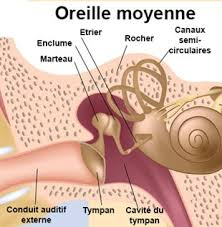
\includegraphics[width=.45\linewidth]{OreilleMoyenne.jpg}
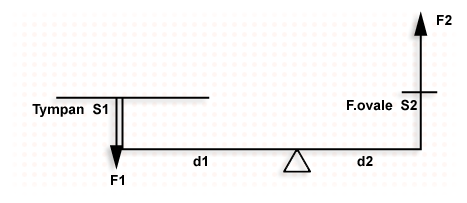
\includegraphics[width=.45\linewidth]{ModeleOreille.png}
\caption{$(a)$ physiologie de l'oreille et $(b)$ Modèle mécanique simplifié des osselets de l'oreille moyenne.}
\end{figure}

Le rôle de l'oreille moyenne est d'optimiser la transmission des ondes acoustiques entre un milieu aérien (le conduit auditif) et un milieu aqueux (la cochlée ou oreille interne).
Pour cela, la solution sélectionnée par la sélection naturelle a consisté à utiliser 3 osselets constituant une sorte de levier reliant ces deux milieux. 
La figure ci-dessus représente ce modèle mécanique de manière très schématique.

On donne les dimensions des bras de levier : $d_1 = 1,3cm$, $d_2 = 1cm$, 
ainsi que la surface du tympan $S_1 = 0.6cm^2$ et celle de la fenêtre ovale $S_2= 0.03cm^2$.
 
\item 
Donnez la relation cinématique entre $u_1$ et $u_2$ (vitesses au niveau du tympan et de la fenêtre ovale).

\item \underline{ En négligeant l'inertie des osselets}, donnez une relation entre les forces $F_1$ et $F_2$  puis entre les pressions $p'_1$ et $p'_2$.

\item Reprendre l'étude de la partie précédente, et donnez une expression du coefficient 
de transmission.

Comparez avec les résultats des questions 10 et 11.





Pour en savoir plus :
\verb| http://www.cochlea.eu/oreille-generalites/oreille-moyenne |
  
\end{enumerate}



 




%%%%%%%%%%%%%%%%%%%%%%%%%%%%%%%%%%%%%%%%%%%%%%%%%%%%%%%%%%%%%%%%%%%%%%%%%%%%%%%%%%%%%%%%%%%%%%%%%%%
\end{document}
%%%%%%%%%%%%%%%%%%%%%%%%%%%%%%%%%%%%%%%%%%%%%%%%%%%%%%%%%%%%%%%%%%%%%%%%%%%%%%%%%%%%%%%%%%%%%%%%%%%

